\documentclass[oneside,monografia]{iftex2020}

% --------------------------------------------------
% Pacotes
% --------------------------------------------------

\usepackage{varwidth}         % Legenda de figuras
\usepackage{fancyvrb}         % Ambiente mono-espaçado
\usepackage{fvextra}          % Melhorias no fancyvrb
\usepackage{textcomp}         % Símbulos extras
\usepackage{tabularx}         % Tabelas

% Ajuste de espaçamento no Verbatim (fancyvrb)
\let\oldverbatim\Verbatim%
\let\oldendverbatim\endVerbatim%
\renewenvironment{Verbatim}%
  {\endgraf\vspace*{-1em}\oldverbatim}%
  {\oldendverbatim\vspace*{-1em}}%

% --------------------------------------------------
% Algoritmos
% --------------------------------------------------
\usepackage[noend]{algpseudocode}
% Comandos para traduzir as instruções do pacote de algoritmos
\algrenewcommand\algorithmicrequire{\textbf{Entrada:}}
\algrenewcommand\algorithmicensure{\textbf{Condição:}}
\algrenewcommand\algorithmicend{\textbf{fim}}
\algrenewcommand\algorithmicif{\textbf{se}}
\algrenewcommand\algorithmicthen{\textbf{então}}
\algrenewcommand\algorithmicelse{\textbf{senão}}
\algrenewcommand\algorithmicfor{\textbf{para}}
\algrenewcommand\algorithmicforall{\textbf{para todo}}
\algrenewcommand\algorithmicdo{\textbf{faça}}
\algrenewcommand\algorithmicwhile{\textbf{enquanto}}
\algrenewcommand\algorithmicrepeat{\textbf{repita}}
\algrenewcommand\algorithmicuntil{\textbf{até que}}
\renewcommand{\Return}{\State \textbf{retorne} }
\let\oldalgorithmic\algorithmic
\let\oldendalgorithmic\endalgorithmic
\renewenvironment{algorithmic}%
  {\hrulefill\vspace*{-0.5em}\oldalgorithmic}%
  {\oldendalgorithmic\vspace*{-1em}\hrulefill}

% --------------------------------------------------
% Comandos personalizados
% --------------------------------------------------
\newcommand{\comando}[1]{\textbf{$\backslash$#1}}
\newcommand{\ifmgtex}[1]{IFMG\TeX}


\addbibresource{referencias.bib}
% Na prática pode ser usado apenas \addbibresource{referencias.bib}
% O comando \addbibresource{referencias.bib} foi usado para mostrar as referências do capítulo de exemplo

% --------------------------------------------------
% Configurações do Documento
% --------------------------------------------------
\titulo{Análise comparativa entre algoritmos de predição de preço para o Bitcoin}
\autor{Mickael Osvaldo de Oliveira}
\local{Bambuí - MG}
\data{15}{Dezembro}{2024}

% Instituição
\instituicao{IFMG}{Instituto Federal Minas Gerais}{Instituto Federal de Educação Ciência e Tecnologia de Minas Gerais}
\unidade{\textit{Campus} Bambuí}
\curso{Bacharel}{Bacharelado}{Engenharia de Computação}

% Orientação
\orientador{Prof. Dr. Ciniro Aparecido Leite Nametala}

% Membros da banca examinadora (além do orientador e coorientador)
\membrobanca{Prof. Dr. Geraldo Henrique Alves Pereira}{IFMG – Campus Bambuí}
\membrobanca{Prof. Dr. Marcos Roberto Ribeiro}{IFMG – Campus Bambuí}

% -------------------------------------------------------
% Elementos Pré-textuais
% -------------------------------------------------------

% --------------------------------------------------
% Resumo e abstract (obrigatórios)
% --------------------------------------------------
\resumo{%
O mercado financeiro atrai a atenção de muitos há séculos, abrangendo ativos variados como arroz, ouro e ações. A flutuação dos preços pode indicar eventos importantes, e prever tais eventos pode determinar o sucesso ou fracasso de um negócio. Diversas técnicas de previsão, como a análise técnica e fundamentalista, surgiram ao longo dos anos. Recentemente, redes neurais, especialmente Long Short-Term Memory (LSTM), têm identificado padrões em séries temporais antes despercebidos. Paralelamente, mercados voláteis como o de criptomoedas emergiram, especialmente após o surgimento do Bitcoin e da tecnologia Blockchain em 2008, oferecendo alternativas para combater a inflação e o controle centralizado. Este estudo visa analisar e comparar algoritmos, em uma base de dados real, que buscam predizer o comportamento dos ativos em mercados voláteis, principalmente no contexto do Bitcoin. Foram utilizadas diferentes abordagens baseadas em descobertas em artigos recentes, proporcionando também variabilidade nos métodos de teste, validação e resultados.
}
\palavraschave{Bitcoin, Redes neurais, previsão de preço.}


% --------------------------------------------------
% Keywords e abstract
% --------------------------------------------------
\abstract{%
The financial market has attracted attention for centuries, encompassing various assets such as rice, gold, and stocks. Price fluctuations can indicate significant events, and predicting these events can determine a business's success or failure. Over the years, various forecasting techniques, such as technical and fundamental analysis, have emerged. Recently, neural networks, especially Long Short-Term Memory (LSTM), have identified previously unnoticed patterns in time series data. Simultaneously, volatile markets like cryptocurrencies have emerged, particularly after the advent of Bitcoin and Blockchain technology in 2008, offering alternatives to combat inflation and centralized control. This study aims to analyze and compare algorithms using a real dataset to predict asset behavior in volatile markets, primarily in the context of Bitcoin. Different approaches based on recent findings were utilized to provide variability in testing methods, validation, and results.
}
\keywords{Bitcoin. Neural networks. Price prediction.}



% Dedicatória (opcional)
\textodedicatoria{%
A minha familia e amigos.

Principalmente a minha mãe, que sempre me apoiou e incentivou a seguir em frente.
}

% Agradecimentos (opcional)
\textoagradecimentos{%
Agradeço a todos que contribuíram para a realização deste trabalho.
}

% Epígrafe (opcional)
\textoepigrafe{%
$B > \frac{1}{n}\sum_{i=1}^{n}x_{i}$ \\
    
}

% Lista de siglas (opcional)
\listasiglas{%
 \begin{itemize}[]
  \item[BTC] -- \textit{Bitcoin}
  \item[FIAT] -- Moeda fiduciária
  \item[ARIMA] -- \textit{Autoregressive Integrated Moving Average}
  \item[ANN] -- \textit{Artificial Neural Network}
  \item[DNN] -- \textit{Deep Neural Network}
  \item[RNN] -- \textit{Recurrent Neural Network}
  \item[LSTM] -- \textit{Long Short-Term Memory}
  \item[BiLSTM] -- \textit{Bidirectional Long Short-Term Memory}
  \item[GRU] -- \textit{Gated Recurrent Unit}
  \item[MAE] -- \textit{Mean Absolute Error}
  \item[MASE] -- \textit{Mean Absolute Scaled Error}
  \item[RMSE] -- \textit{Root Mean Square Error}
  \item[MAPE] -- \textit{Mean Absolute Percentage Error}
  \item[$R^2$] -- \textit{R-squared}
 \end{itemize}
}


% Ficha catalográfica (obrigatória)
\ficha{ficha_catalografica}

% --------------------------------------------------
% Folha de aprovação (obrigatória)
% --------------------------------------------------
% Assinaturas e QRCode recortados do documento SEI
%\assinaturas{assinaturas}

% -------------------------------------------------------
% Elementos opcionais
% -------------------------------------------------------

% Lista de figuras (opcional)
\listafiguras
% Lista de quadros (opcional)
% \listaquadros
% Lista de tabelas (opcional)
\listatabelas
% Lista de algoritmos (opcional)
% \listaalgoritmos
% Lista de códigos (opcional)
% \listacodigos

\begin{document}

% -------------------------------------------------------
% Gera elementos pré-textuais
% -------------------------------------------------------
\maketitle

% -------------------------------------------------------
% Capítulo: Introdução
% -------------------------------------------------------
\chapter{Introdução} \label{cap:introducao}

A história da matemática na predição de preços remonta ao trabalho pioneiro \textit{Théorie de la Spéculation} de \textcite{Bachelier} \cite{Fama1965,Fama,Courtault}. É fundamentado no conceito do movimento Browniano, 
fenômeno que descreve o deslocamento errático de partículas em um fluido, que o autor utiliza como analogia para o comportamento imprevisível dos preços de ativos no mercado financeiro. 
Essa ideia deu origem à teoria conhecida como \textit{Random Walk} (Caminhar Aleatório), que, posteriormente, serviu de base para outras modelagens, como a de \textcite{blacksholes}.

Dentre os ramos que compõem a projeção de preços, destacam-se as análises técnicas e fundamentalistas.
A análise técnica busca predizer os preços futuros baseados em análises passadas de preço, volume e contratos abertos em opções \cite{Pring}.
Por outro lado, a análise fundamentalista se baseia em estimar o valor intrínseco dos ativos, ou seja, encontrar o preço justo por fundamentos do projeto, preços passados, situação atual e oportunidades futuras \cite{Ahmed}.

O \textit{Bitcoin} foi introduzido por \textcite{Nakamoto}, entidade desconhecida sob o pseudônimo de Satoshi Nakamoto. 
É considerada a primeira moeda digital implemementada que transaciona de maneira totalmente descentralizada, sem a necessidade de uma autoridade central, como um banco ou governo. 
Para isso, utiliza uma tecnologia denominada \textit{Blockchain}, que funciona como um livro-caixa em uma estrutura de dados distribuída e imutável \cite{Ledger}. Podem ser trocados por outras moedas ou ativos, como o Real, em plataformas de negociação de ativos digitais chamadas \textit{Exchanges} \cite{FakeExchanges}.

A troca desses ativos gera um histórico de transações como em qualquer mercado financeiro,
porém, consideravelmente mais volátil, devido à falta de lastro das moedas fiduciárias (Fiat) tradicionais. 
Tendo em vista o caminhar aleatório do mercado, a análise preditiva não deve ser considerada uma tarefa trivial, mas pode ser facilitada com o uso de técnicas de aprendizado de máquina.
Nos dias atuais, segundo \textcite{Fang}, os analistas de mercado têm feito uso não somente destes métodos, mas também de outros modelos computacionais convecionais ou híbridos, que têm por objetivo prever os preços, obtendo sucesso especialmente no contexto das criptomoedas \cite{Atsalakis}.

\section{Justificativa}
As redes neurais artificiais (RNAs) tornaram-se uma peça fundamental na sociedade moderna. Por isso, novas técnicas surgem a cada dia para resolver múltiplos problemas, 
muitas vezes, não solucionáveis por humanos \cite{Good}.
Por outro lado, o mercado de ativos baseados em criptografia cresce exponencialmente, 
sendo muito utilizado como reserva de valor, meio de pagamento e uma forma de diversificação de investimentos \cite{Sousa}.

Então, justifica-se este trabalho, pois essas duas tecnologias convergem
para um mundo cada vez mais digital; a união delas pode até mesmo ser intrínseca a muitas criptomoedas.
A previsão de preços em mercados financeiros não é recente; entretanto, ativos com alta volatilidade, como o Bitcoin, ainda apresentam potencial para operações lucrativas \cite{Tri}.
Assim, este estudo busca explorar dois temas relevantes atualmente, especialmente sob a perspectiva da engenharia de computação, contribuindo para o avanço do conhecimento em áreas exploradas.


\section{Proposta}

Este estudo tem como proposta analisar e avaliar algoritmos voltados para previsão de preços, a fim de verificar sua lucratividade em operações usando um dos mais famosos criptoativos, o Bitcoin.
Os modelos foram avaliados de acordo com suas previsões em um cenário real de variação de preço, estruturados por meio de uma série temporal histórica. A pesquisa utilizou essa mesma base de dados e manteve os métodos de pré-processamento fixos, variando no contexto da aplicação apenas o algoritmo de previsão.
Isto foi feito de forma a manter as condições de experimentação para todos os algoritmos, garantindo, assim, que a diferença estivesse apenas no funcionamento de cada um.
Os dados foram obtidos por meio dos registros de negociações reais na \textit{Exchange}
 Binance, que contém informações como o preço, o volume e o número de transações realizadas entre janeiro e setembro de 2020.
As arquiteturas exploradas incluem a ARIMA, LSTM, BiLSTM e GRU.

\subsection{Objetivo geral}

Comparar o desempenho de algoritmos de predição de preço no contexto do Bitcoin.

\subsection{Objetivos específicos}

Para atingir o objetivo principal, foram necessários os seguintes objetivos específicos:
\begin{itemize}
    \item Desenvolver a estrutura computacional necessária para selecionar, implementar e realizar previsões por meio de ferramentas tecnológicas adequadas (como linguagens de programação, métodos de extração e armazenamento de dados, geradores gráficos e demais ferramentas necessárias);
    \item Avaliar RNAs e compará-los frente aos \textit{Benchmarks} de interesse, a fim de determinar qual tem melhor desempenho;
    \item Explorar possíveis variações em métodos conhecidos, visando adaptá-los a um novo cenário;
    \item Avaliar a rentabilidade desses métodos através de métricas em uma base de dados real.
\end{itemize}

\section{Estrutura do documento}

Este trabalho está estruturado em seis capítulos. Após a introdução, são apresentados os fundamentos teóricos necessários para a compreensão das principais técnicas empregadas na metodologia. 
Desse modo, o capítulo \ref{cap:fundamentacao_teorica} aborda conceitos de criptomoedas e séries temporais, fornecendo uma introdução à análise de dados, explorando artigos relacionados 
à estrutura do mercado e à predição de preços. 
Além disso, é apresentado o estado da arte em relação às RNAs e suas aplicações no contexto do mercado financeiro.

O Capítulo \ref{cap:metodologia} apresenta a metodologia, organizada de acordo com a sequência de implementação da solução.
No capítulo \ref{cap:resultados}, são descritos os resultados e discussões dos experimentos realizados.
O capítulo \ref{cap:conclusao} oferece uma conclusão que abrange as principais contribuições, limitações da pesquisa e propostas para trabalhos futuros.

\chapter{Fundamentação teórica} \label{cap:fundamentacao_teorica}


Este capítulo oferece o arcabouço teórico necessário para a compreensão da pesquisa em sí. 
Portanto, serão abordados conceitos fundamentais relacionados
a criptomoedas, \textit{blockchain}, redes neurais e previsão de séries temporais.
\section{Bitcoin}
\label{secao:bitcoin}

A ideia de Ativos Digitais descentralizados baseados em criptografia, ou criptomoedas, foi marcada por inúmeras tentativs anteriores, contudo,
só foi implementada com o advento da \textit{Blockchain} \cite{Moi}.
Que é referida por \textcite{Yuan} como um registro compartilhado distribuído, no qual a verificação, armazenamento, manutenção e transmissão dos dados são baseados na confiança mútua entre as partes, estabelecida por meio de algoritmos matemáticos.
Tal estrutura é formada por blocos que contêm um conjunto 
de transações, cada bloco possui um identificador exclusivo chamado Hash,
gerado a partir das informações presentes no bloco, incluindo o do anterior. 
Esse encadeamento de blocos cria uma sequência contínua e cronológica, na qual os blocos são ligados ao anterior formando uma cadeia \cite{Blockchain}.

\begin{figure}[!htb] \centering
  \caption{Representação da Blockchain} \label{figura:imageBlock}
  \begin{varwidth}{\linewidth}
    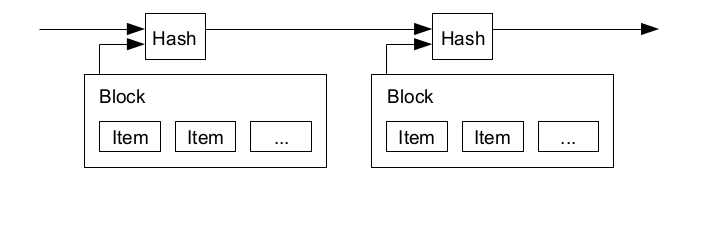
\includegraphics[width=8cm]{figuras/imageBlock.png}
    \fonte{\citefonte{Nakamoto}.}
  \end{varwidth}
\end{figure}

O primeiro e mais conhecido ativo desse setor se chama Bitcoin, definido como um dinheiro eletrônico negociado diretamente entre pares, sem passar por uma instituição financeira \cite{Nakamoto}.
Desde emtão, tem se publicado diversos artigos que buscam explorar essa nova area de mercado, segundo \textcite{Sousa}, as tecnologias baseadas em \textit{Blockchain} são mais mais rápidas, ágeis e seguras que seus pares centralizados. 
Por isso, esse nicho vem ganhando bastante espaço na mídia, assim, atraindo interesse por parte de investidores individuais e fundos. 

Cada \textit{Bitcoin} é subdividido em 100 milhões de unidades menores chamadas Satoshis, ou simplismente "Sats".
Seu armazenamento é feito em uma carteira digital ciptografada de maneira assimétrica Offline chamadas \textit{Cold Wallets} ou Online em serviços de \textit{Hot Wallets} \cite{wallet}.
A transferência ocorre por prova de trabalho, um validador chamado de minerador é responsável por resolver um problema matemático de dificuldade variável, além disso, serve como nó que confere a operação de outros mineradores e garante a integridade da rede.
Quando o problema é resolvido adiciona-se um bloco de transação na Blockchain. Em troca, o minerador recebe uma recompensa em \textit{Bitcoins} \cite{pow}.
A dificuldade da prova de trabalho é ajustada automaticamente pelo \textit{Hashrate}, indicador que mede a quantidade de poder computacional necessário à mineração. Quanto maior o \textit{Hashrate}, mais difícil é encontrar o próximo bloco, regulando o tempo entre a adição de novos blocos a rede, mantendo uma média de 10 minutos.

\begin{figure}[!htb] \centering
    \caption{Prova de trabalho} \label{figura:imageNonce}
    \begin{varwidth}{\linewidth}
      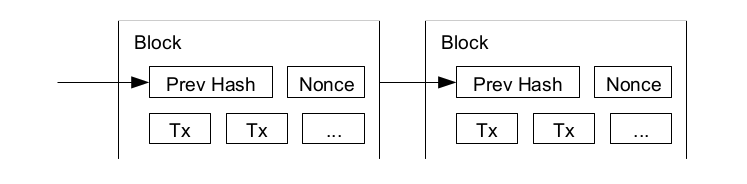
\includegraphics[width=8cm]{figuras/nonce.png}
      \fonte{\citefonte{Nakamoto}.}
    \end{varwidth}
  \end{figure}

A cada quatro anos, o número de \textit{Bitcoins} gerados por bloco é reduzido pela metade, evento conhecido como \textit{Halving}.
O fator de redução confere a moeda uma escassez programada, limitada a 21 milhões de unidades, que a torna deflacionária.
Ativos baseados em ciptografia e a inteligência artificial são parte fundamental da \textit{Web 3.0}, considerada como a terceira geração da internet \cite{web3}.
Recentemente os contratos inteligentes, \textit{DeFi} (Finanças Descentralizadas), \textit{NFTs} (Tokens Não Fungíveis) e a inteligência artificial generativa ensaiam uma nova era de aplicações e serviços.

\begin{figure}[!htb] \centering
    \caption{Livros lançados por assunto} \label{figura:imagengram}
    \begin{varwidth}{\linewidth}
      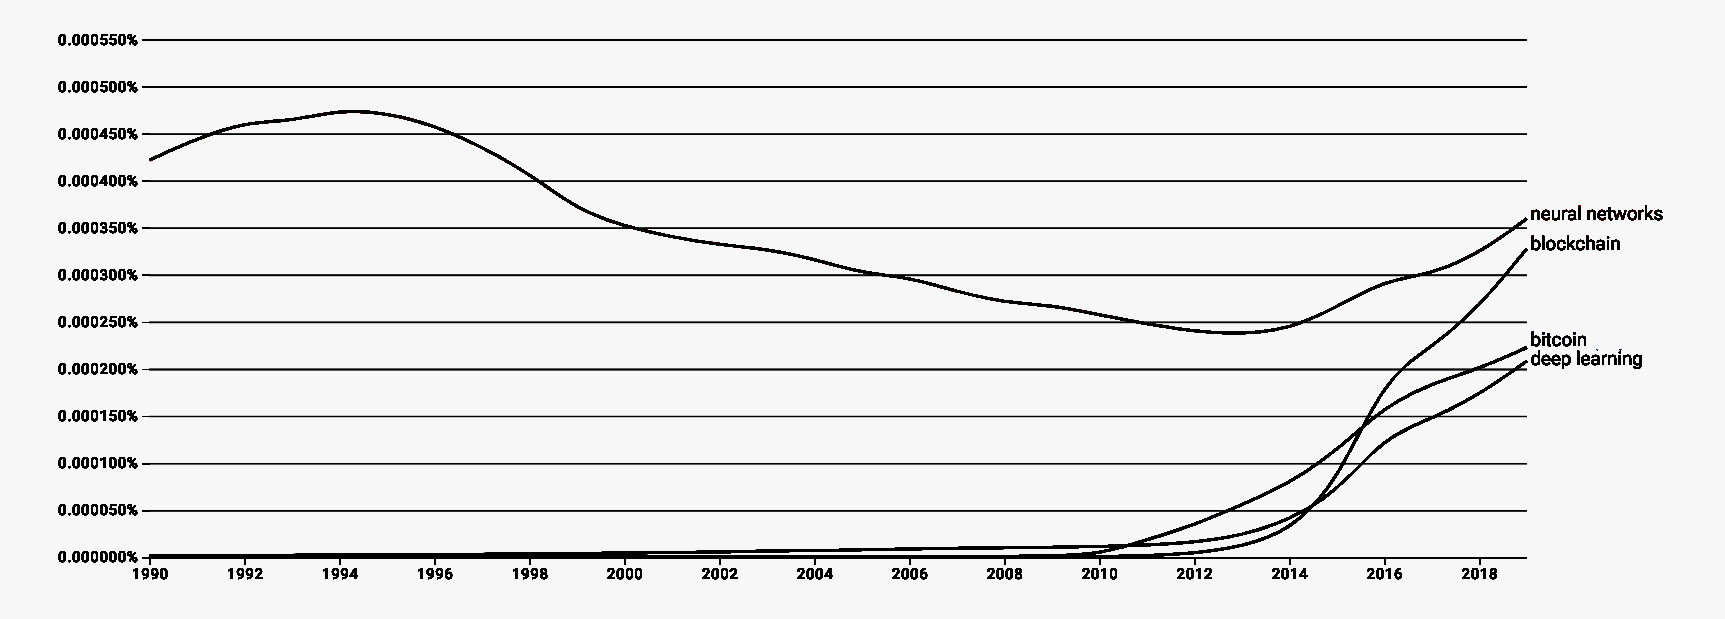
\includegraphics[width=15cm]{figuras/ngram.png}
      \fonte{\cite{books}}
    \end{varwidth}
  \end{figure}

No contexto de negociação do \textit{Bitcoin} a mais conhecida das \textit{Exchanges} é a Binance, que opera em diversos países e possui um volume de transações diário de bilhões de dólares.
Com uma liquidez alta o Spread, diferença entre o preço de compra e venda, é baixo, o que representa o valor bem acurado com o oferecido no mercado.
Além disso, existem Sites de comparação de preços. os mais populares são o CoinGecko e CoinMarketCap, funcionando
como portais que classificam as plataformas, moedas e até a situação atual do mercado através de índices.


% em 29 de jun. 2024
\begin{table}[!htb]
  \caption{Exchanges com maior volume e confiabilidade} \label{tabela:lista_produtos}
  \begin{tabularx}{\textwidth}{l|c|c|c} \hline
    Exchange      & Volume 24h (BTC) & Score Coingecko & Score CoinMarketCap  \\ \hline
    Binance (Global)      & 135.157      & 10/10        & 9,9/10 \\
    Bybit         & 44.720      & 10/10        & 7.6/10  \\
    HTX (Huobi)       & 34.250     & 9/10        & 6.9/10  \\ \hline
  \end{tabularx}
  \fonte{Elaborado pelo autor, 2024.}
\end{table}

%\section{\textit{Aprendizado de máquina}} \label{sec:apc}

\section{\textit{Autoregressive Integrated Moving Average}} \label{sec:arima}

O ARIMA (\textit{Autoregressive Integrated Moving Average}) tem suas raízes na econometria e na estatística.
Sua história remonta ao trabalho pioneiro de \textcite{Box}, no qual os autores introduziram uma abordagem sistemática para identificar, estimar e diagnosticar modelos de séries temporais, conhecida como metodologia Box-Jenkins \cite{Arima}.
Combinam três componentes principais: auto-regressão (AR), diferenciação (I) e médias móveis (MA). A componente AR descreve a relação entre uma observação atual e observações passadas, enquanto a componente MA modela a dependência entre uma observação e erros de previsão passados. 

\section{Redes neurais} \label{sec:redes neurais}

A teoria de Redes Neurais Artificiais (ANNs) teve início com os estudos realizados por \textcite{Rosenblatt}.
Este autor desenvolveu o \textit{Perceptron}, um algoritmo fundamentado nas teorias formuladas por \textcite{McCulloch, hebb} que modelavam as conexões dos neurônios no cérebro de animais \cite{Good}.
Apesar de suas vantagens, à época o \textit{Perceptron} era capaz apenas de resolver problemas linearmente separáveis, como destacado por \textcite{Minsky}. Este fato os impedia de ser utilizados em muitos problemas reais,
o que causou uma crise no estudo da área como um todo. Fato que mais tarde foi contornado por \textcite{Rumelhart}, que juntos desenvolveram o algoritmo de \textit{Backpropagation} para treinar a arquitetura denominanda de \textit{Multilayer Perceptron} (MLP).

\begin{figure}[!htb] \centering
  \caption{Camadas de uma MLP} \label{figura:multilayer}
  \begin{varwidth}{\linewidth}
    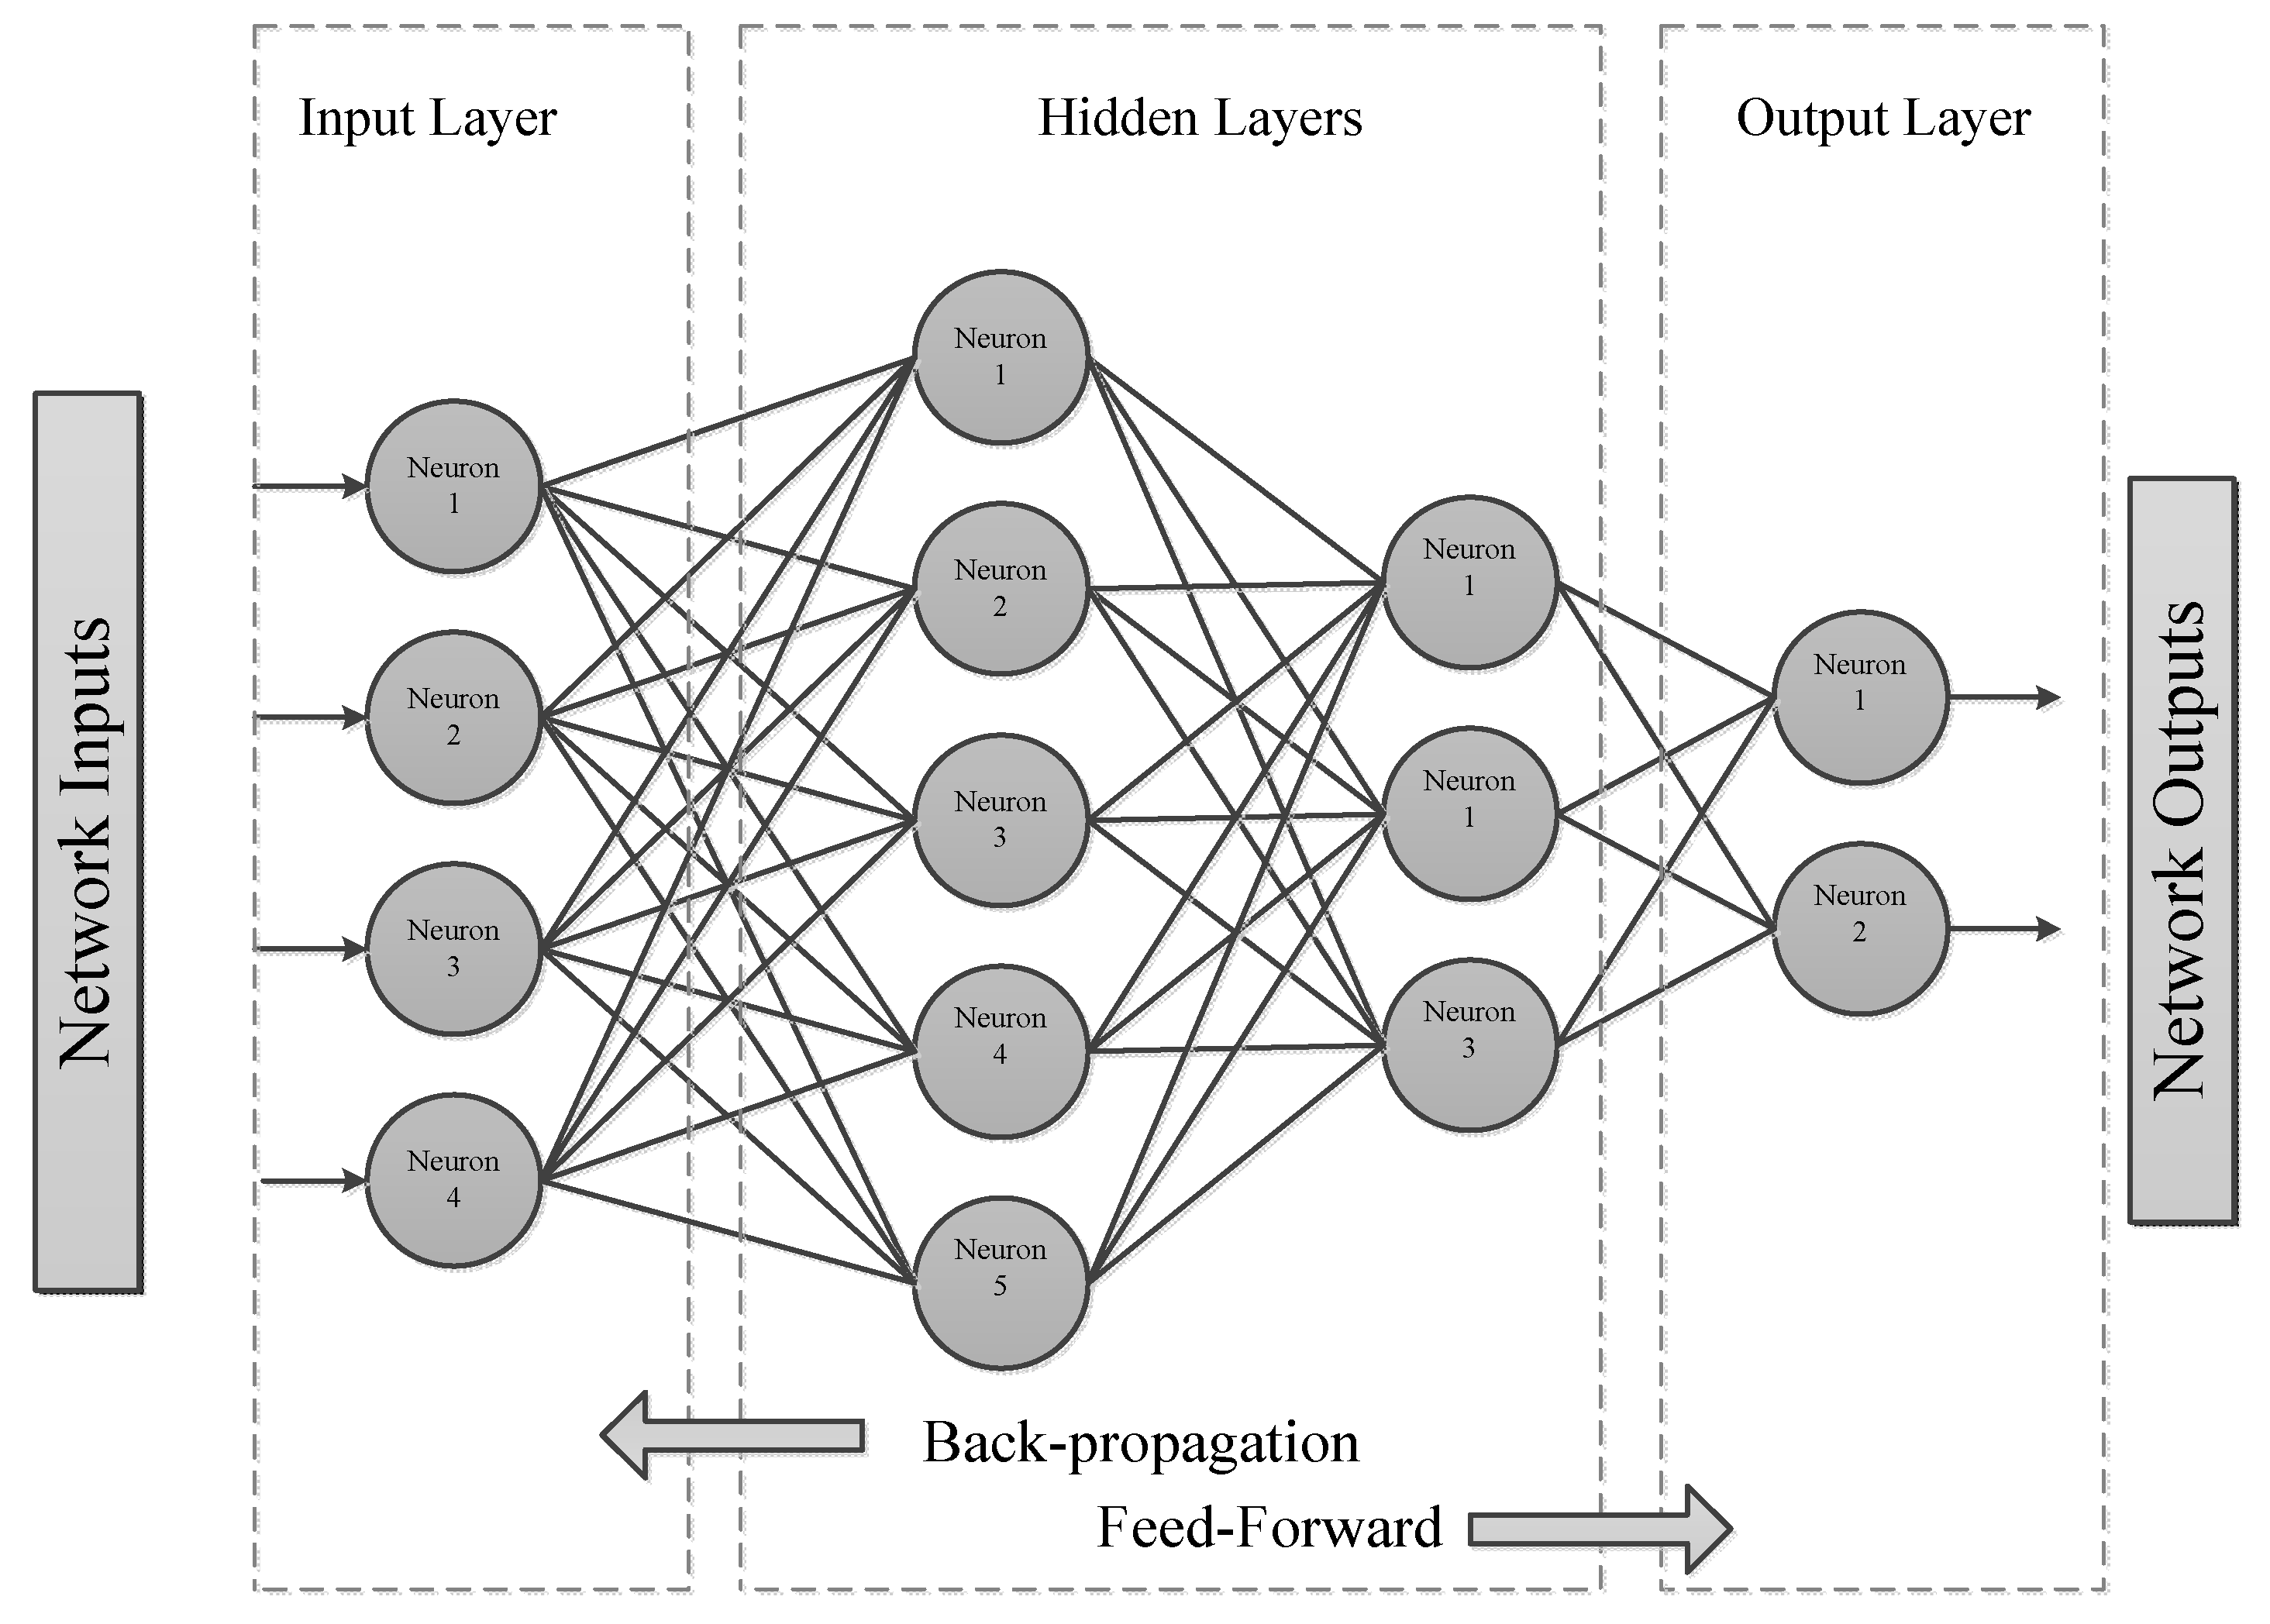
\includegraphics[width=12cm]{figuras/mlp.png}
    \fonte{\cite{multilayer}}
  \end{varwidth}
\end{figure}

Após esse início, os algoritmos baseados em redes neurais evoluíram de forma a se tornar cada vez mais precisos e especializados em tarefas distintas.
Pode-se dar destaque neste contexto aos modelos
que podem ser combinados para gerar complexas arquiteturas no que hoje é conhecido como \textit{Deep Neural Networks} (DNNs) ou \textit{Deep Learning} \cite{Good}. Como se verifica nas revisões bibliográficas mais recentes, tais arqioteturas vêm demonstrando grande capacidade de auxiliar na resolução de problemas de classificação, previsão e análise de sentimentos \cite{Hanc}.

\subsection{\textit{Recurrent Neural Networks}} \label{sec:rnn}

Das arquiteturas apresentadas é possível notar que representam grafos cujas arestas não formam ciclos na mesma fase.
Quando tal condição é subvertida e se estabelecem ciclos, obtem-se redes neurais recorrentes (RNNs)\cite{graves}.
Embora essa diferença possa parecer trivial, as implicações devem ser consideradas na implementação.
Enquanto uma MLP percorre apenas entre vetores de entrada e saída, \textcite{graves} destaca que uma RNN, a princípio, consegue mapear todo o histórico de entradas para cada saída. Atuando como uma memória que persiste de resultados passados para execuções futuras. 
Pode-se então inferir a utilidade desses modelos em dados sequenciais $x^{(1)}$, ..., $x^{(\tau)}$ \cite{Good}.

\begin{figure}[!htb] \centering
  \caption{Camadas cíclicas de uma RNN} \label{figura:rnn}
  \begin{varwidth}{\linewidth}
    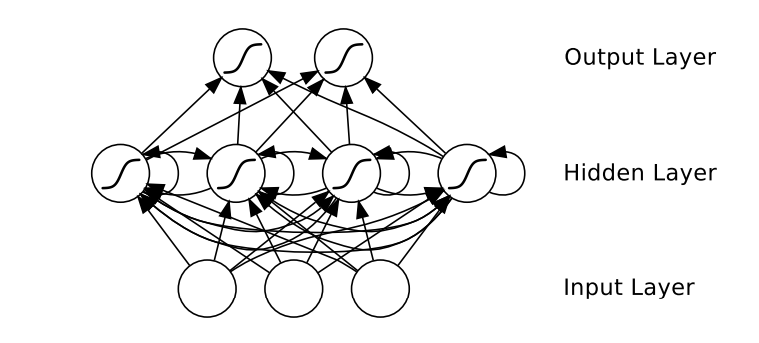
\includegraphics[width=12cm]{figuras/rnn.png}
    \fonte{\cite{graves}}
  \end{varwidth}
\end{figure}

Armazenar dependências ao longo das iterações é certamente o principal desafio matemático na implementação de redes recorrentes.
Segundo \cite{graves}, o problema consiste em que gradientes propagados por muitas execuções tendem a desaparecer (na maioria dos casos) ou explodir (raramente, mas com grande impacto na otimização).
Mesmo assumindo que os parâmetros da rede sejam estáveis, a dificuldade surge à medida que em que o modelo converge e os 
\textit{Steps\footnote{ O salto no aprendizado (ou \textit{step}) da rede se tornar exponencialmente menor pode ser explicado observando as mínimas ou máximas locais e globais em uma função n-dimensional. Fato demonstrado no livro de \textcite{stewart}.}} se tornam menores \cite{Good}.
Uma maneira de lidar com a dispersão dos gradientes é projetar um modelo que opere em múltiplas escalas temporais \cite{Bengio} e realizar o 
\textit{Clipping\footnote{\textit{Clipping} é uma técnica que consiste em limitar a magnitude dos gradientes a um intervalo válido, impedindo que ultrpassem valores predefinidos.}} dos gradientes para evitar as explosões \cite{Exp}.

\subsection{\textit{Long-Short Term Memory}} \label{sec:lstm}
Os modelos baseados em células de memória \textit{Long-Short Term Memory} (LSTM) foram desenvolvidos por \textcite{Hoch}, fazem parte de uma seleta classe dos modelos sequênciais de RNNs controladas (\textit{gated RNNs}).
A ideia é produzir um \textit{loop} entre uma mesma unidade, o que leva a caminhos onde o gradiente pode perdurar por muitas iterações.
Novas abordagens introduziram o peso nesse \textit{loop} condicionado ao contexto em vez de fixo, sendo então controlado por outra unidade oculta \cite{Gers}. 
Assim, a escala pode ser alterada dinamicamente, mesmo que uma LSTM tenha parâmetros fixos, a escala pode mudar com base na sequência 
de entrada, pois as constantes de tempo são determinadas pelo próprio modelo.

\begin{figure}[!htb] \centering
  \caption{Diagrama de blocos de uma LSTM} \label{figura:lstm}
  \begin{varwidth}{\linewidth}
    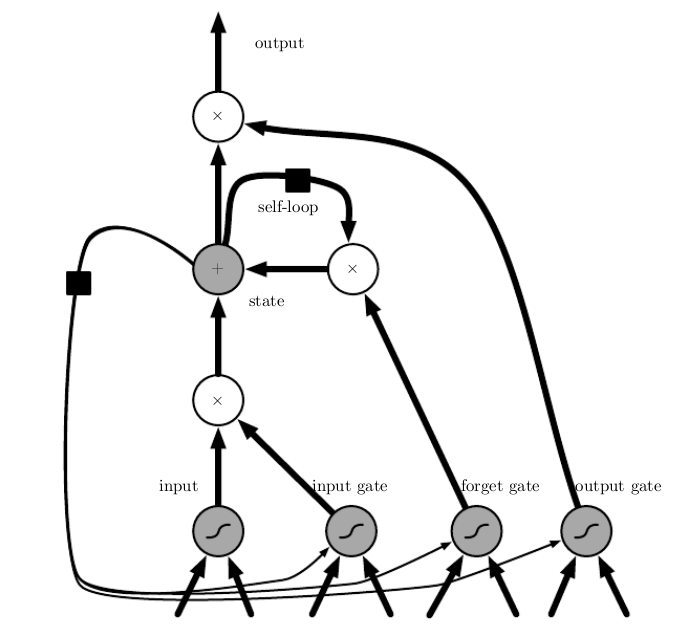
\includegraphics[width=10cm]{figuras/lstm.png}
    \fonte{\cite{graves}}
  \end{varwidth}
\end{figure}

\subsection{\textit{Bidirectional Long Short-Term Memory}} \label{sec:bilstm}

A ideia de adicionar camadas em direções opostas nas redes recorrentes foi proposta por \textcite{Schuster} e denominadas redes bidirecionais.
Essa técnica posteriormente foi adaptada nos estudos de \textcite{bilstm}, que propuseram uma LSTM Bidirecional, ou \textit{Bidirectional Long Short-Term Memory} (biLSTM).
Sua estrutura é formada por duas LSTMs: 
uma recebendo as entradas à frente enquanto outra recebe na direção oposta.
O intuito é que a saída de cada unidade influencie indiretamente em sua contraparte, de forma que os gradientes não dispersem conforme o tempo.


\subsection{\textit{Gated Recurrent Unit}} \label{sec:gru}
A \textit{Gated Recurrent Unit} (GRU) é um tipo de RNN introduzida por \textcite{Cho}.
Sua estrutura é semelhante às LSTMs, mas, têm uma arquitetura minimalista e, portanto, são computacionalmente mais eficientes. 
Utilizam dois tipos principais de portas (\textit{gates}) para controlar o fluxo de informações dentro da unidade: a porta de reset (\textit{Reset gate}) e a porta de atualização (\textit{update gate}).

\begin{figure}[!htb] \centering
  \caption{Estrutura de uma GRU} \label{figura:gru}
  \begin{varwidth}{\linewidth}
    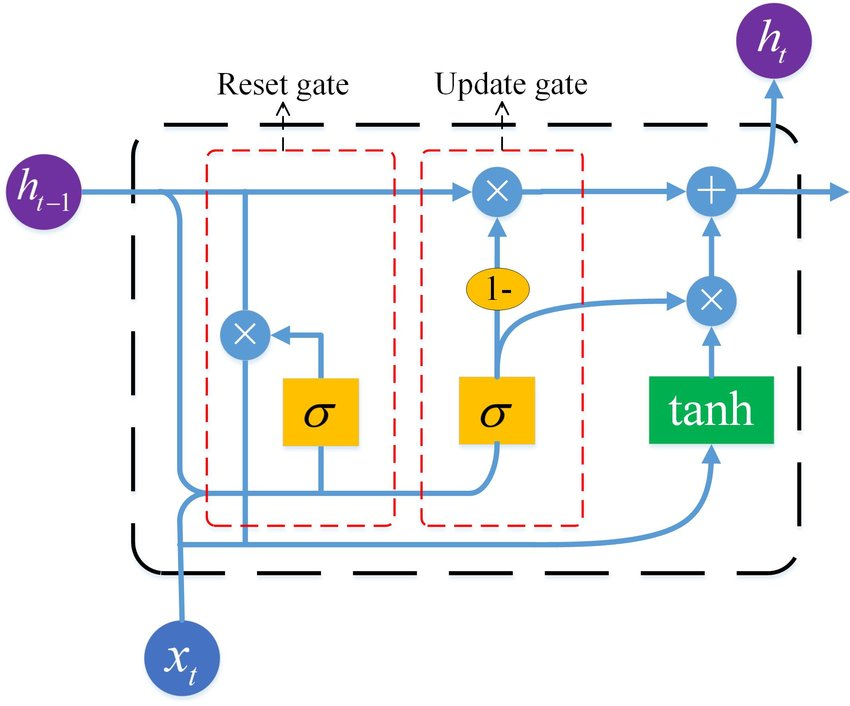
\includegraphics[width=10cm]{figuras/gru.png}
    \fonte{\cite{gru-image}}
  \end{varwidth}
\end{figure}

\section{\textit{Séries temporais}} \label{sec:temp}
Séries temporais são conjuntos de dados intrinsecamente relacionados ao tempo, sua natureza ordenada e agrupada em intervalos regulares
torna a sequência cronológica fundamental \cite{Esling}. Alguns desses conjuntos possuem ciclos repetitivos em períodos distintos, chamadas sazonalidades. 
Possuem inúmeras aplicações, representando vendas, preços de ações e variações nos mais diversos contextos.

O número de amostras e a correlação de eventos são fatores primordiais que definem a complexidade da análise.
\textcite{Nison} destaca que já no século XVIII, os japoneses desenvolveram uma forma de
visualização de séries temporais popularmente conhecida como \textit{Candlestick}.
Desde então, o comportamento que denota sua variação, representada em ativos como no mercado financeiro, intriga economistas, estastísticos e professores de finanças \cite{Fama}

%\subsection{Previsão de preços} \label{sec:previsao}

%Prever preços não é algo necessariamente novo ou exclusivo de mercados digitais. Porém, utilizar os recursos computacionais atuais aliados a técnicas especificas para séries temporais podem proporcionar uma maior assertividade.

\section{Estado da arte} \label{sec:estado}

Em artigos recentes \textcite{Fer} obtiveram sucesso em prever preços do Bitcoin para o dia seguinte com modelos LSTM. Autores como \textcite{Tri} combinam métodos bayesianos, processamento de sinais e redes neurais a fim de prever o preço em múltiplos intervalos de tempo.

\textcite{Zhang} compilam resultados de modelos para previsão de preço, detecção de bolha e construção de portfólio que podem aumentar a lucratividade no âmbito das criptomoedas.
A variedade de algoritmos empregados e a diversidade em resultados obtidos demonstram a complexidade do problema, assim, reforça a necessidade de se explorar diferentes abordagens.

\begin{table}[!htb]
  \scriptsize
  \caption{Comparação entre estudos na área} \label{tabela:lista_estudos}
  \begin{tabularx}{\textwidth}{l|X|X|X|X|X} \hline
    Pesquisadores & Ativo & Entradas & Saídas & Modelos & Métricas \\ \hline
    \cite{lstmvsgru} & Bitcoin & Preço & Preço médio & LSTM, GRU & SMAPE \\ \hline
    \cite{Fer} & Bitcoin & Preço & Preço & LSTM & RMSE \\ \hline
    \cite{Siami} & Ações & Preço & Preço& ARIMA, LSTM, BiLSTM & RMSE \\ \hline
    \cite{Tri} & Bitcoin & Preço ou indicadores& Preço & DANN, LSTM, BiLSTM, CNN-BiLSTM & RMSE, MAE, MAPE \\ \hline
    Autor & Bitcoin & Preço, trocas e volume & Preço & ARIMA, LSTM, BiLSTM e GRU & MSE, MAPE, MASE, $R^2$ \\ \hline
  \end{tabularx}
  \fonte{Elaborado pelo autor, 2024.}
\end{table}


\chapter{Metodologia} \label{cap:metodologia}


Utilizando como base \textcite{pesquisa}, pode-se dizer que a pesquisa adota
uma abordagem quantitativa e experimental, ou seja, visa analisar e contrastar o desempenho
de diferentes algoritmos em condições controladas. A natureza aplicada do estudo busca não
apenas compreender as nuances de cada algoritmo, mas também oferecer \textit{insights} para a seleção
e implementação dos mais eficazes. A metodologia descritiva permite uma análise detalhada
dos resultados obtidos, destacando as diferenças significativas entre os modelos avaliados.

\subsection{Solução proposta} \label{sec:solucao}

\begin{figure}[!htb] \centering
    \caption{Fluxo de implementação da solução} \label{figura:proposta}
    \begin{varwidth}{\linewidth}
      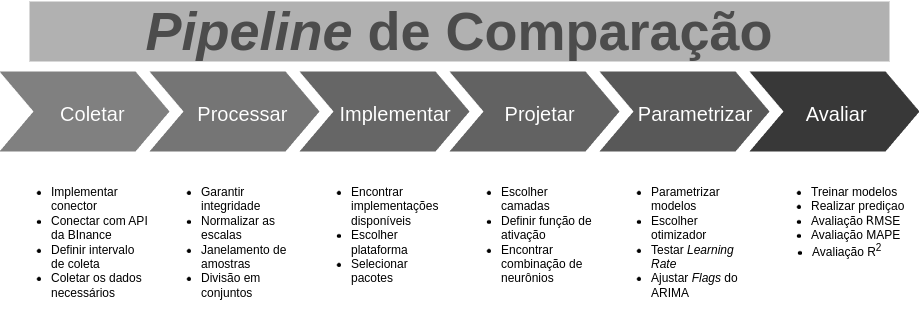
\includegraphics[width=16cm]{figuras/proposta.png}
      \fonte{Elaborado pelo autor, 2024.}
    \end{varwidth}
  \end{figure}

\section{Coleta de dados} \label{sec:coleta}
A coleta de dados ou obtenção de \textit{Datasets} envolve inicialmente selecionar locais como APIs, bancos de dados online ou arquivos históricos que forneçam os dados em um formato estruturado, como JSON, CSV ou TOML.
Mas, é possível estabelecer um processo de coleta automatizada através de \textit{Crawlers} ou \textit{Web Scrapping} para extrair as informações brutas.
Independente da escolha sempre é preciso realizar um projeto de dados, que envolve a definição de quais informações são relevantes e sua correlação, para isso, existem métodos como a análise exploratória de dados (EDA) e a visualização de dados como no \textit{Pair Plot}.
A tabela \ref{tab:amostras} apresenta um exemplo de amostras que foram coletadas.

\section{Pré processamento} \label{sec:preprocessamento}
No processo de análise de dados, é comum que os dados brutos apresentem inconsistências, como valores ausentes, duplicados ou mal formatados. 
Essas imperfeições comprometem a eficácia dos modelos, antes de enviar os dados para o treinamento, é crucial assegurar que estejam completos, formatados e escalonados de maneira adequada.
A essa etapa dá-se o nome de pré-processamento.

\begin{table}[!htb]
    \caption{Amostras da base de dados coletada} \label{tab:amostras}
    \begin{tabularx}{\textwidth}{X|X|X|X}
    \hline
    Data (GMT-3) & Volume & Trocas & Preço \\ \hline
    2020-01-01 00:00:00   & 1959651.83      & 2811            & 7228.5         \\ \hline
    2020-01-01 00:15:00   & 1225409.70      & 1897            & 7237.15        \\ \hline
    2020-01-01 00:30:00   & 1469869.68      & 2163            & 7221.27        \\ \hline
    2020-01-01 00:45:00   & 1012436.07      & 1466            & 7225.01        \\ \hline
    2020-01-01 01:00:00   & 1102372.81      & 1985            & 7219.09        \\ \hline
    \end{tabularx}
    \fonte{Elaborado pelo autor, 2024.}
\end{table}

\subsection{Validação de completude} \label{sec:completude}
Para verificar a completude dos dados, foi utilizada uma função nativa do \textit{Pandas}, garantindo que todas as entradas estejam presentes na base.
Embora o conector a realize na captura, é necessário uma verificação adicional a cada análise para assegurar a qualidade das amostras. 
Caso exista valores ausentes, é possível utilizar métodos como a interpolação para estimar os valores faltantes e preenchê-los.

\subsection{Normalização} \label{sec:normalizar}
Em um \textit{Dataset} multivariado é comum que os valores estejam em escalas distintas, no caso do \textit{Bitcoin}, o preço e o volume variam em ordens de grandeza superiores ao número absoluto de transações.
Isso se deve à própria natureza da dimensão dos dados, por isso, é necessário padronizar as variáveis para que o modelo não seja enviesado.
Uma das técnicas de normalização mais famosas ajusta as colunas para um intervalo que esteja entre o máximo e o mínimo valor encontrado, assim,  é chamada de \textit{MinMaxScaller}.
\begin{equation}
    {X_{Scalled} = \frac{X-X_{min}}{X_{max}-X_{min}}}
    \label{eq:scalled}
\end{equation}

Na equação acima, x é o valor original da variável, min(x) é o valor mínimo encontrado na coluna e max(x) o valor máximo.
Ao final obtemos o equivalente dimensionado da respectiva linha, ajustado em escala de 0 a 1.

\subsection{Limitações e diferenças entre algoritmos} \label{sec:limitacao}
O processamento de dados em diferentes algoritmos, seja no aprendizado de máquina ou modelagem estatística, requer um dimensionamento de dados contendente com as necessidades e limitações de cada método.
Ao utilizar redes neurais, é comum que o modelo consiga lidar bem com múltiplas variáveis e forneça um arcabouço robusto de soluções adquiridas durante o treinamento.

Por outro lado, modelos como a regressão linear são tradicionalmente univariados, significando que modelam uma única variável de interesse.
Outra característica é que não são treinados no sentido tradicional, em vez disso, ajustam seus parâmetros diretamente aos valores históricos, requerendo dados estacionários.
Ou seja, as entradas devem ser ligeiramente adaptadas às necessidades do modelo.

\subsection{Janelamento} \label{sec:janelamento}

Ao se trabalhar com séries temporais é comum a separação dos dados em segmentos menores
 a fim de capturar a dinâmica ao longo do tempo.
Uma dessas técnicas envolve a criação de janelas deslizantes, na qual um intervalo fixo de observações é utilizado para prever os próximos valores.
No contexto de redes neurais, essa abordagem é bastante útil, pois permite que o modelo capture padrões locais e evolutivos, aproveitando o poder da memória da rede para entender sequências.

Entretanto, quando se trata de modelos estatísticos, o processo de segmentação é geralmente feito de maneira incremental.
Em vez de usar uma janela deslizante de tamanho fixo, o modelo pode se beneficiar de uma janela expansiva, onde todos os dados disponíveis até um determinado ponto são utilizados para fazer a previsão seguinte.
Isso torna justa a comparação, visto que o máximo de informação disponível é utilizada para cada previsão.

\begin{figure}[!htb] \centering
    \caption{Técnicas de janelamento} \label{figura:window}
    \begin{varwidth}{\linewidth}
      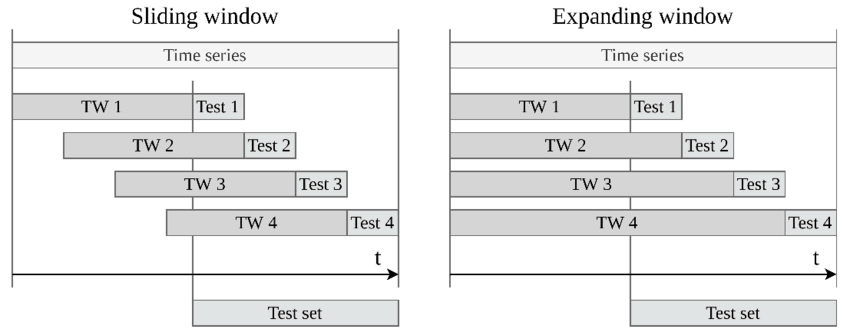
\includegraphics[width=12cm]{figuras/window.png}
      \fonte{\citefonte{Sliding}.}
    \end{varwidth}
\end{figure}
  

\subsection{Divisão em conjuntos} \label{sec:divisao}
Para avaliar a eficácia dos modelos de aprendizado supervisionado, a base de dados é dividida em três subconjuntos: treinamento, validação e teste.
O conjunto de treinamento é usado para ajustar os pesos do modelo, enquanto o de validação serve para otimizar os hiperparâmetros com base na função de perda.
Após o limite de épocas o conjunto de teste, que contém dados que o modelo ainda não viu, é utilizado para verificar a capacidade de generalizar seu desempenho. A etapa não é necessária para o ARIMA, que ajusta seus parâmetros diretamente sobre todos os dados.

\begin{figure}[!htb] \centering
    \caption{Divisão de dados} \label{figura:train_test}
    \begin{varwidth}{\linewidth}
      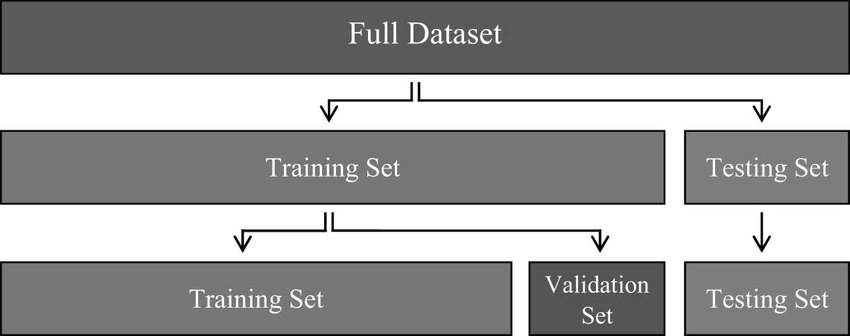
\includegraphics[width=12cm]{figuras/train_test.png}
      \fonte{\citefonte{Sliding}.}
    \end{varwidth}
\end{figure}

\section{Implementação} \label{sec:implementacao}
Todos os modelos foram desenvolvidos utilizando a linguagem de programação \textit{Python} versão 3.10 \cite{ramalho}, juntamente com as bibliotecas \textit{Pandas} e \textit{Numpy} \cite{Data}. 
Na implementação de redes neurais foram utilizados os \textit{Frameworks} Keras 3.10 e TensorFlow 2.10 \cite{maosaobra}, essas ferramentas podem ser adaptadas para processamento paralelo em GPU, mas, para isso a placa de video deve ter suporte a CUDA, tecnologia de codigo aberto da NVIDIA.
O ARIMA foi feito e otimizado com base no Pmdarima, biblioteca que implementa o modelo de forma eficiente.

\section{Arquitetura} \label{sec:arquitetura}
Cada modelo foi implementado de acordo com as especificações de suas respectivas arquiteturas, a seguir, são apresentadas as principais características de cada um.

\begin{table}[h!] \label{tabela:lstm_struct}
    \caption{Estrutura do modelo baseado em LSTM}
    \begin{tabularx}{\textwidth}{X|X|X|c|X} \hline
    Camada & Tipo & Neurônios & Função de Ativação & Parâmetros \\ \hline
    1 & LSTM                    & 16 & Tangente Hiperbólica                           & 1.280                  \\ \hline
    2 & LSTM                    & 32 & Tangente Hiperbólica                            & 6.272                  \\ \hline
    3 & LSTM                    & 32 & Tangente Hiperbólica                            & 8.320                  \\ \hline
    4 & Densa                   & 16 & Tangente Hiperbólica                            & 528                    \\ \hline
    5 & Densa                   & 1  & Tangente Hiperbólica                           & 17                     \\ \hline
    \end{tabularx}
    \fonte{Elaborado pelo autor, 2024.}
\end{table}

\begin{table}[h!] \label{tabela:gru_struct}
    \caption{Estrutura do modelo baseado em GRU}
    \begin{tabularx}{\textwidth}{X|X|X|c|X} \hline
    Camada & Tipo & Neurônios & Função de Ativação & Parâmetros \\ \hline
    1                   & GRU                     & 75                     & -                           & 18.000                 \\ \hline
    2                   & GRU                     & 30                     & -                           & 9.630                  \\ \hline
    3                   & GRU                     & 30                     & -                           & 5.580                  \\ \hline
    4                   & Densa                   & 1                      & -                           & 31                     \\ \hline
    \end{tabularx}
    \fonte{Elaborado pelo autor, 2024.}
\end{table}

\begin{table}[h!] \label{tabela:bidirectional_struct}
    \caption{Estrutura do modelo baseado em camadas Bidirecionais}
    \begin{tabularx}{\textwidth}{X|X|X|c|X} \hline
    Camada & Tipo & Neurônios & Função de Ativação & Parâmetros \\ \hline
    1                   & Bidirectional            & 256                    & -                           & 135.168                \\ \hline
    2                   & Bidirectional            & 128                    & -                           & 164.352                \\ \hline
    3                   & Densa                   & 32                     & Tangente Hiperbólica                           & 4.128                  \\ \hline
    4                   & Densa                   & 1                      & -                           & 33                     \\ \hline
    \end{tabularx}
    \fonte{Elaborado pelo autor, 2024.}
\end{table}
    





\section{Configuração} \label{sec:configuracao} 
Os parâmetros da rede foram definidos de forma geral e aplicados uniformemente a todos os modelos avaliados. A configuração padrão adotada é descrita detalhadamente na Tabela \ref{tabela:parametros}.

\begin{table}[h!]
    \caption{Configuração dos parâmetros das redes neurais} \label{tabela:parametros}
    \begin{tabularx}{\textwidth}{X|X} \hline
    Parâmetros & Valores \\ \hline
    Batch         & 32               \\ \hline
    Épocas         & 1000              \\ \hline
    Otimizador               & Nadam ($\eta=0{,}0001$; $\beta_1=0{,}85$; $\beta_2=0{,}989$; $\epsilon=10^{-6}$)             \\ \hline
    Função de perda          & MSE              \\ \hline
    \end{tabularx}
    \fonte{Elaborado pelo autor, 2024.}
\end{table}

\section{Avaliação} \label{sec:avaliacao}
Para avaliar a acurácia dos modelos de previsão, é preciso separar em duas categorias: aprendizado de máquina e estatística.
No aprendizado de máquina (supervisionado) é possivel validar diretamente na função de perda, que no caso é a MSE, enquanto nos estatísticos o cálculo é inerente à fórmula.

Na comparação final será feita uma combinação de métricas estatísticas 
que permitem analisar tanto a precisão quanto a robustez das previsões.
As métricas escolhidas para essa avaliação são: 
Mean Squared Error (MSE), Mean Absolute Percentage Error (MAPE), Mean Absolute Scaled Error (MASE) e o Coeficiente de Determinação (R²). Cada uma dessas métricas fornece uma perspectiva única sobre a qualidade das previsões e será descrita a seguir.

\begin{equation}
    \text{MSE} = \frac{1}{n} \sum_{t=1}^{n} (\hat{y}_t - y_t)^2
\end{equation}

Calcula a média dos quadrados da diferença entre os valores previstos ŷ e os valores reais y. Penaliza erros maiores mais severamente, já que a diferenças é elevada ao quadrado

\begin{equation}
    \text{MAPE} = \frac{1}{n} \sum_{t=1}^{n} \left|\frac{y_t - \hat{y}_t}{y_t}\right|
\end{equation}

Média dos erros percentuais absolutos na série, padronizando a análise para que seja possível comparar diferentes escalas ou unidades.
Quando a diferença entre y e ŷ é dividida por y, obtêm-se o percentual, que é então normalizado pela média. Como o somatório de valores decimais pode ser confuso, alguns autores sugerem multiplicar cada resultado por 100 para facilitar a interpretação.


\begin{equation}
    \text{MASE} = \frac{\frac{1}{n} \sum_{t=1}^{n} |y_t - \hat{y}_t|}{\frac{1}{n-1}\sum_{t=2}^{n} |y_t - y_{t-1}|}
\end{equation}

A principal função dessa métrica é comparar os erros do modelo original com a predição \textit{Naive} (ingênua), que simplesmente prevê o valor anterior.
Caso o erro seja maior ou igual a 1, o modelo é considererado tão ruim quanto duplicar valores.
A fórmula basicamente compara a média absoluta de erro (MAE) dos modelos, então, é uma média comum com módulo.

\begin{equation}
    R^2 = 1 - \frac{\sum_{t=1}^{n} (y_t - \hat{y}_t)^2}{\sum_{t=1}^{n}(y_t - \bar{y})^2}
\end{equation}

O erro $R^2$, também chamado de coeficiente de determinação, representa a proporção da variabilidade dos dados que é explicada pelo modelo, variando de 0 a 1, sendo 1 o ajuste perfeito.
O $y_t$ define os valores reais, $\hat{y}_t$ os valores preditos e $\bar{y}$ é a média dos valores observados. O numerador contém a soma dos erros ao quadrado entre os valores reais e preditos (erro do modelo), enquanto o denominador é a soma da variabilidade total dos dados

\section{Materiais e Tecnologias} \label{sec:materiais}
Para a realização deste trabalho, 
foram utilizados um processador Intel Core i5-12500H e
uma placa de vídeo NVIDIA GeForce RTX 3050 de 4GB com suporte a CUDA 12
Um total de 16GB de memória RAM foram utilizados para armazenas os tensores, parâmetros e janelamento em memória dos dados. 
O sistema operacional foi o Linux Pop! OS 20.04 e o desenvolvimento foi feito no editor Visual Studio Code, utilizando Python 3.10. As bibliotecas empregadas incluíram Pandas e Numpy para manipulação e computação de dados, e Matplotlib e Seaborn para visualização. Para aprendizado de máquina e redes neurais, foram utilizados os frameworks Keras e TensorFlow, e o modelo ARIMA foi implementado com a biblioteca Pmdarima.

\chapter{Resultados e discussão} \label{cap:resultados}

Os resultados deste capítulo referem-se oa gráfico de preço,volume e transações do \textit{Bitcoin}, em intervalos de 15 minutos, ao longo de 2020 (GMT -3). Foram utilizados dados da Binance no par BTC/USDT com uma implementação própria chamado BTools, cobrindo todo o ano (01/01/2020 a 31/12/2020), no qual representa 365 dias e 10000 entradas. 
Esse conjunto de dados então foi armazenado em um arquivo CSV e posteriormente dividido em memória para o treinamento dos modelos supervisionados e ajustados para os estatísticos.

\section{Tratamento e pré processamento de dados}
O \textit{Dataset} não continha valores nulos ou faltantes, porém, foi necessário realizar a normalização através do método MinMaxScaler devido a diferentes ordens de grandeza entre as variáveis.
Para o aprendizado supervisionado, os conjuntos de treinto, teste e validação foram divididos em 70\%, 20\% e 10\% respectivamente. 
O janelamento utilizado foi de 24 entradas (6 horas) para prever o próximo valor de preço.

No ARIMA foi utilizado o método de auto arima para encontrar os melhores parâmetros p, d e q com base no primeiro janelamento.

\chapter{Conclusão} \label{cap:conclusao}

Neste estudo foram exploradas diferentes abordagens de modelagem para a previsão do preço do Bitcoin em intervalos de 15 minutos, comparando métodos estatísticos e redes neurais recorrentes. 
O \textit{Dataset} continha dados de preço, volume e trocas de janeiro a setembro de 2020, um período de alta volatilidade. Desse modo, ncluiu uma análise de desempenho de modelos como ARIMA, GRU, LSTM e BiLSTM, aplicados às séries temporais propostas.
As arquiteturas supervisionadas e estatisticas foram separadas levando em consideração as limitações de cada uma, como a necessidade de janelamento e a quantidade de \textit{Features}.

O modelo ARIMA, conhecido por sua robustez em séries lineares, obteve os melhores resultados no contexto, superando ligeiramente os modelos de rede neural ao apresentar previsões precisas e consistentes.
Porém, o fato das neurais não performarem tão bem quanto seu competidor estatístico não significa que elas não possam ser utilizadas, mas sim que precisam de mais ajustes e engenharia de \textit{Features} para melhorar a previsão.

Como continuidade para este trabalho, sugere-se a investigação de abordagens híbridas que combinem a capacidade preditiva do ARIMA com a sensibilidade temporal das redes neurais. Além disso, é possível expandir os testes para outros períodos e ativos financeiros. 

Outras recomendações incluem:

\begin{itemize}
    \item Realizar ajustes nas configurações das redes neurais, como o número de camadas, unidades ocultas, função de ativação e hiperparâmetros
    \item Identificar arquiteturas ainda mais adaptadas à volatilidade;
    \item Aplicar a metodologia a outras criptomoedas, intervalos de tempo e ativos financeiros para validar a generalização dos resultados;
    \item Comparar o desempenho com técnicas mais recentes, considerando diferentes condições de mercado e intervalos temporais.
\end{itemize}

Portanto, este estudo cumpre os objetivos propostos e contribui para a compreensão do comportamento do mercado de criptomoedas e a aplicação de técnicas de previsão de séries temporais.


% -------------------------------------------------------
% Elementos pós-textuais
% -------------------------------------------------------
\postextual

% -------------------------------------------------------
% Referências bibliográficas
% -------------------------------------------------------

\printbibliography[notkeyword=exemplo]
% Na prática pode ser usado apenas \printbibliography
% O comando \printbibliography[notkeyword=exemplo] foi usado para não mostrar as referências do capítulo de exemplo

\end{document}
